% !TeX spellcheck = en_US
\documentclass[french]{yLectureNote}

\title{Mécanique}
\subtitle{Mécanique du point}
\author{Paulhenry Saux}
\date{\today}
\yLanguage{Français}

\professor{S.Deheuvels}%sebastien.deveuhels.irap.omp.eu

\usepackage{graphicx}%----pour mettre des images
\usepackage[utf8]{inputenc}%---encodage
\usepackage{geometry}%---pour modifier les tailles et mettre a4paper
%\usepackage{awesomebox}%---pour les boites d'exercices, de pbq et de croquis ---d\'esactiv\'e pour les TP de PC
\usepackage{tikz}%---pour deiffner + d\'ependance de chemfig
\usepackage{tkz-tab}
\usepackage{chemfig}%---pour deiffner formules chimiques
\usepackage{chemformula}%---pour les formules chimiques en \'equation : \ch{...}
\usepackage{tabularx}%---pour dimensionner automatiquement les tableaux avec variable X
\usepackage{awesomebox}%---Pour les boites info, danger et autres
\usepackage{menukeys}%---Pour deiffner les touches de Calculatrice
\usepackage{fancyhdr}%---pour les en-t\^ete personnalis\'ees
\usepackage{blindtext}%---pour les liens
\usepackage{hyperref}%---pour les liens (\`a mettre en dernier)
\usepackage{caption}%---pour la francisation de la l\'egende table vers Tableau
\usepackage{pifont}
\usepackage{array}%---pour les tableaux
\usepackage{lipsum}
\usepackage{yFlatTable}
\usepackage{multicol}
\usepackage{cancel}
\usepackage{xcolor}
\newcommand\Ccancel[2][black]{\renewcommand\CancelColor{\color{#1}}\cancel{#2}}
\newcommand{\Lim}[1]{\lim\limits_{\substack{#1}}\:}
\renewcommand{\vec}{\overrightarrow}
\newcommand{\norm}[1]{||\vec{#1}||}
\newcommand{\dd}[0]{\mathrm{d}}
\newcommand{\ddp}[0]{\partial}
%\DeclareMathOperator\arctanh{arctanh}
\DeclareMathOperator\grad{grad}
\begin{document}

%\titleOne
\setcounter{chapter}{7}
	\chapter{Puissance, travail et énergie - Méthode}
\section{Exprimer le travail d'une force}
Il faut peut \^etre d'abord découper le mouvement en plusieurs parties pour avoir des déplacements plus simples à analyser.
\subsection{Méthode générale}
\begin{enumerate}
 \item On applique la formule : $W_{AB}(\vec{F_i}) = \int_{C,AB}\vec{F}\cdot \dd \vec{r}$
 \item On projette le vecteur sur les axes de notre base : $W_{AB}(\vec{F_i}) = \int_{C,AB}(F_x\vec{e_x}+F_y\vec{e_y}+F_z\vec{e_z})\cdot \dd \vec{r}$
 \item On réécrit le déplacement élémentaire dans la base considérée (souvent la cartésienne) : $W_{AB}(\vec{F_i}) = \int_{C,AB}(F_x\vec{e_x}+F_y\vec{e_y}+F_z\vec{e_z})\cdot (\dd x \vec{e_x} + \dd y \vec{e_y} + \dd z \vec{e_z})$\marginInfo{Souvent le déplacement se fait selon un ou 2 axes seulement, il est donc inutile d'écrire toutes les composantes de la base considérée.}
 \item On développe l'expression en supprimant les produits scalaires dont les résultats sont nuls, c'est à dire tous ceux entre 2 vecteurs orthogonaux :
 $W_{AB}(\vec{F_i}) = \int_{C,AB}F_x\vec{e_x}\cdot \dd x \vec{e_x}+F_y\vec{e_y}\cdot \dd y \vec{e_y}+F_z\vec{e_z}\cdot \dd z \vec{e_z}$
 \item On obtient une somme de produits scalaires dont les vecteurs sont colinéaires et unitaires. Les produits scalaires sont donc égaux à 1. Il nous reste :
  $W_{AB}(\vec{F_i}) = \int_{C,AB}F_x\cdot \dd x +F_y\cdot \dd y+F_z\cdot \dd z$
  \item On peut séparer les intégrales pour les traiter séparément :
  $W_{AB}(\vec{F_i}) = \int_{C,AB}F_x\cdot \dd x +\int_{C,AB}F_y\cdot \dd y+\int_{C,AB}F_z\cdot \dd z$
  \item On intègre chaque intégrale entre les coordonnées x, y ou z selon l'intégrale du début et de fin du chemin.
\end{enumerate}
\subsection{Force constante}
\criticalInfo{Force constante}{Pour qu'une force puisse \^etre qualifiée de constante, sa norme doit l'\^etre mais cela ne suffit pas ! Il faut aussi que la direction et le sens le soient aussi !. Autrement dit, il faut que le vecteur force soit constant et non sa norme.}
Pour une force constante, on peut sortir le vecteur Force de l'intégrale. On obtient alors $W_{AB}(\vec{F_i}) = \vec{F}\cdot\int_{C,AB} \dd \vec{r} = \vec{F}\cdot\vec{AB}$. En effet, la somme de tous les déplacements élémentaires entre A et B donne le vecteur $\vec{AB}$.\marginCritical{Attention, la somme de tous les \emph{vecteurs} de déplacement élémentaire donne bien le vecteur $\vec{AB}$ mais la somme des déplacement élémentaires donne la longueur du chemin !} On peut alors simplement faire le produit scalaire.
\subsection{Force de m\^eme direction que le mouvement}
On réécrit $W_{AB}(\vec{F_i}) = \int_{C,AB}\vec{F}\cdot \dd \vec{r}$ comme $W_{AB}(\vec{F_i}) = \int_{C,AB}F\frac{\vec{v}}{\norm{v}}\cdot \dd \vec{r}$. Comme le vecteur vitesse divisé par sa norme est unitaire et colinéaire au déplacement élémentaire, on obtient $W_{AB}(\vec{F_i}) = \int_{C,AB}F \dd r$. Si la norme du vecteur est constante, on peut la sortir de l'intégrale et obtenir : $W_{AB}(\vec{F_i}) = F \times ||C_{AB}||$ avec $||C_{AB}||$ la longueur du chemin.
\subsection{Force orthogonale au mouvement}
La force est orthogonale à $\dd\vec{r}$, donc le produit scalaire est nul, ainsi que le travail.
\subsection{Exemple d'une force constante}
On étudie la trajectoire d'un skateur dans un skatepark. On cherche à déterminer le travail du vent $\vec{F_v}$ sur sur le skateur, en fonction de sa direction et des angles des tremplins.

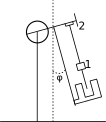
\includegraphics[scale=0.5]{schema}

On va découper le trajet en plusieurs parties et calculer le travail sur chacune d'entre elle.\marginTips{On va dans cette exemple appliquer la méthode générale, m\^eme si l'on pourrait très bien utiliser la méthode, plus simple du cas où la force est constante\dots}
\subsubsection{Sur AB}
\begin{enumerate}
\item On applique la formule : $W_{AB}(\vec{F_v}) = \int_{C,AB}\vec{F_v}\cdot \dd \vec{r}$
 \item On projette le vecteur sur les axes de notre base : $W_{AB}(\vec{F_v}) = \int_{C,AB}(F_v\times\cos(a)\vec{e_x}-F_v\times\sin(a)\vec{e_y})\cdot \dd \vec{r}$
 \item On réécrit le déplacement élémentaire dans la base considérée (souvent la cartésienne) : $W_{AB}(\vec{F_v}) = \int_{C,AB}(F_v\times\cos(a)\vec{e_x}-F_v\times\sin(a)\vec{e_y})\cdot (\dd x \vec{e_x} + \dd y \vec{e_y})$
 \item On développe l'expression en supprimant les produits scalaires dont les résultats sont nuls, c'est à dire tous ceux entre 2 vecteurs orthogonaux :
 $W_{AB}(\vec{F_v}) = \int_{C,AB}F_v\times\cos(a)\vec{e_x}\cdot \dd x \vec{e_x}-F_v\times\sin(a)\vec{e_y}\cdot \dd y \vec{e_y}$
 \item On obtient une somme de produits scalaires dont les vecteurs sont colinéaires et unitaires. Les produits scalaires sont donc égaux à 1. Il nous reste :
  $W_{AB}(\vec{F_v}) = \int_{C,AB}F_v\times\cos(a) \dd x -F_v\times\sin(a) \dd y$
  \item On peut séparer les intégrales pour les traiter séparément :
  $W_{AB}(\vec{F_v}) = \int_{C,AB}F_v\times\cos(a) \dd x +\int_{C,AB}-F_v\times\sin(a) \dd y$
  \item On intègre chaque intégrale entre les coordonnées x, y ou z selon l'intégrale du début et de fin du chemin.
  \begin{itemize}
   \item Le vecteur $\vec{F_v}$ est constant, on peut donc l'extraire de l'intégrale : $\int_{C,AB}F_v\times\cos(a) \dd x = F_v\times\cos(a)\int_{C,AB} \dd x = F_v\times\cos(a)\times AB$\marginCritical{On a effectué cette opération uniquement car la force est constante et de m\^eme direction que le chemin ! Si l'une de ces conditions n'est pas remplie, on ne peut pas le faire !}
   \item Il n'y a pas de déplacement selon $y$ sur cette section. La deuxième intégrale est donc nulle.
  \end{itemize}
\end{enumerate}
On obtient donc : $W_{AB}(\vec{F_v}) = F_v\times\cos(a)\times AB$.

On remarque qu'on retrouve bien l'expression pour le travail d'une force constante, car $F_v\times\cos(a)\cdot AB = \vec{F_v}\cdot \vec{AB}$
\subsubsection{Sur BC}
Les étapes 1 à 6 sont les m\^eme que précédemment. En effet, seul le chemin change.
\begin{enumerate}
\setcounter{enumi}{6}
  \item On intègre chaque intégrale entre les coordonnées x, y ou z selon l'intégrale du début et de fin du chemin.
  \begin{itemize}
   \item Le vecteur $\vec{F_v}$ est constant, on peut donc l'extraire de l'intégrale : $\int_{C,BC}F_v\times\cos(a) \dd x = F_v\times\cos(a)\int_{C,BC} \dd x$
   \item On intègre : $ F_v\times\cos(a)\int_{B}^C \dd x = F_v\times\cos(a)[x]_{B}^C$
   \item Il faut maintenant trouver les coordonnées $x$ de B et C. Pour B, c'est la distance AB et pour C c'est $AB + \sin(b)\times BC$
   \item On peut maintenant faire le calcul : $F_v\times\cos(a)[x]_{B}^C = F_v\times\cos(a)\times(AB + \sin(b)\times BC) - F_v\times\cos(a)\times(AB) = F_v\times\cos(a)\times(\sin(b)\times BC)$
   \item De la m\^eme façon, on obtient le travail pour le déplacement selon $y$\marginTips{On remarque que les coordonnées $y$ du point B sont 0 et celles de C sont $\cos(b)\times BC$} : $-F_v\times\sin(a)[x]_{B}^C = -F_v\times\sin(a)\times(\cos(b)\times BC) - (-F_v\times\sin(a)\times 0)) = -F_v\times\sin(a)\times(\cos(b)\times BC)$
  \end{itemize}
\end{enumerate}
Finalement, le travail vaut sur cette section : $F_v\times\cos(a)\times(\sin(b)\times BC) -F_v\times\sin(a)\times(\cos(b)\times BC) = F_v\times BC(\cos(a)\sin(b)-\sin(a)\cos(b))$\marginInfo{Ici aussi, $\cos(a)\sin(b)-\sin(a)\cos(b)$ vaut le $\cos$ de l'angle entre le vent et le chemin, i.e $\cos(\frac{\pi}{2}-b+a)$. En effet, à l'aide de formules trigonométriques, on peut montrer l'égalité\dots}

On remarque qu'il est nul seulement si les angles $a$ et $b$ sont égaux, ce qui correspond à la situation où le vent est orthogonal à la pente montante.
\subsubsection{Sur DE}
Les étapes 1 à 6 sont les m\^eme que précédemment. En effet, seul le chemin change.
\begin{enumerate}
\setcounter{enumi}{6}
  \item On intègre chaque intégrale entre les coordonnées x, y ou z selon l'intégrale du début et de fin du chemin.
  \begin{itemize}
   \item Le vecteur $\vec{F_v}$ est constant, on peut donc l'extraire de l'intégrale : $\int_{C,BC}F_v\times\cos(a) \dd x = F_v\times\cos(a)\int_{C,BC} \dd x$
   \item On intègre : $ F_v\times\cos(a)\int_{B}^C \dd x = F_v\times\cos(a)[x]_{B}^C$
   \item Il faut maintenant trouver les coordonnées $x$ de D et E. Pour D, c'est la distance AD' et pour E c'est $AD' + \cos(c)\times DE$
   \item On peut maintenant faire le calcul : $F_v\times\cos(a)[x]_{D}^E = F_v\times\cos(a)\times(AD' + \cos(c)\times DE) - F_v\times\cos(a)\times(AD') = F_v\times\cos(a)\times(\cos(c)\times DE)$
   \item De la m\^eme façon, on obtient le travail pour le déplacement selon $y$\marginTips{On remarque que les coordonnées $y$ du point D sont $-\sin(c)DE$ et celles de E sont $0$} : $-F_v\times\sin(a)[x]_{D}^E = -F_v\times\sin(a)\times(0) - (-F_v\times\sin(a)\times (-\sin(c)DE))) = F_v\times\sin(a)\times(\sin(c)DE)$
  \end{itemize}
\end{enumerate}
Finalement, le travail vaut sur cette section : $F_v\times\cos(a)\times(\cos(c)\times DE)+F_v\times\sin(a)\times(\sin(c)DE) = F_vDE(\cos(a)\cos(c)+\sin(a)\sin(c))$\marginInfo{On remarque que pour que le vent aide le plus possible, il faut que les angles $a$ et $c$ soient égaux. Ainsi, le vent et la pente sont dans la m\^eme direction.}
\subsubsection{Somme}
Pour obtenir le travail sur ces portions (on a exclu le moment où le skater décolle et se trouve en l'air entre les points C et D), on fait la somme des 3 travaux trouvés : $W(\vec{F_v}) = F_v\times\cos(a)\times AB + F_v\times BC(\cos(a)\sin(b)-\sin(a)\cos(b)) + F_vDE(\cos(a)\cos(c)+\sin(a)\sin(c))$.
\subsection{Exemple d'une force de frottement}
On étudie les forces de frottement $F_f = -\alpha \vec{v}$liées aux roues d'un skateur lors du parcours ci-dessous. Remarquons que la norme du vecteur est constante.

Comme dans l'autre exemple, nous allons séparer le parcourt en 3 parties, la ligne AB, l'arc de cercle BC et la ligne CD\marginInfo{Je ne vais pas traiter le chemin CD car c'est la m\^eme situation que la ligne AB}.

\includegraphics[scale=0.6]{schema2}
\subsubsection{Sur AB}
Appliquons la méthode :
\begin{enumerate}
 \item On applique la formule : $W_{AB}(\vec{F_i}) = \int_{C,AB}\vec{F}\cdot \dd \vec{r}$
 \item On écrit le vecteur $\vec{F_f}$ en fonction d'un vecteur unitaire lié au vecteur vitesse : $W_{AB}(\vec{F_i}) = \int_{C,AB}(-\alpha \frac{\vec{v}}{\norm{v}})\cdot \dd \vec{r}$
 \item On peut sortir $-\alpha$ de l'intégrale qui est constant : $W_{AB}(\vec{F_i}) = -\alpha\int_{C,AB}( \frac{\vec{v}}{\norm{v}})\cdot \dd \vec{r}$
 \item Remarquons que la somme sur le chemin $AB$ de $\frac{\vec{v}}{\norm{v}}\cdot \dd \vec{r} = \frac{1}{\norm{v}}\times \norm{v}\times \dd r \times \cos(0) = \dd r$ donne la somme de la distance parcourue et donc la longueur du chemin. On peut donc simplifier l'intégrale : $W_{AB}(\vec{F_i}) = -\alpha\times ||C_{AB}|| = AB$.
\end{enumerate}
\subsubsection{Sur BC}
De la m\^eme façon, on obtient $W_{AB}(\vec{F_i}) = -\alpha\times ||C_{AB}||$\marginInfo{Ici, $||C_{AB}||$ vaut la distance l'arc $BC$, que l'on peut calculer en connaissant le rayon R et la hauteur du point $C$.}
\subsection{Force de rappel du ressort : Force non constante}
Appliquons la méthode pour la force de rappel du ressort. Dans un déplacement après $l_0$, on a :
\begin{flalign*}
W_{C(AB)} (\vec{F_r}) &= \int_{C(AB)} \vec{F_r} \cdot \mathrm{d}\vec{r}\\
&= \int\vec{F_r} \cdot (\mathrm{d}x\vec{e_x} + \mathrm{d}y\vec{e_y} + \mathrm{d}z\vec{e_z})\\
&= \int\vec{F_r} \cdot \mathrm{d}x\vec{e_x}\\
&=  \int^{x_b}_{x_a}-kx \mathrm{d}x\\
&= -k[\frac{x^2}{2}]^{x_b}_{x_a} \\
&= -\frac{1}{2}k(x_b^2-x_a^2)
\end{flalign*}
%\section{Relation entre Force conservative et énergie potentielle}
%\subsection{Déterminer une force à partir de son énergie potentielle}
\section{Déterminer une énergie potentielle à partir d'une force}
\subsection{Avec le travail}
On utilise la relation entre le travail et la variation d'énergie potentielle :$\delta W=-\dd E_p$.
\subsubsection{Force électrostatique}
Exemple : Considérons une force d'attraction entre 2 particules : $\vec{f} = \frac{q_aq_b}{4\pi\varepsilon_0r^2}\vec{e_{\rho}}$ dans un repère polaire. Le déplacement élémentaire dans ce type de repère est $\dd\rho\vec{e_{\rho}}+\rho\dd\varphi\vec{e_{\varphi}}$.

On a : \begin{flalign*}
\delta W &= \vec{f}\cdot \dd\vec{r}\\
&= \vec{f}\cdot \dd(\dd\rho\vec{e_{\rho}}+\rho\dd\varphi\vec{e_{\varphi}})\\
&= \frac{q_aq_b}{4\pi\varepsilon_0r^2} \dd \rho
\end{flalign*}
En effet, la force s'exprime seulement avec $\vec{e_{\rho}}$, donc le produit scalaire avec $\vec{e_{\varphi}}$ est nul et celui avec $\dd\rho\vec{e_{\rho}}$ donne bien $\dd\rho$. Une fois l'expression trouvée, on peut calculer l'énergie potentielle :
\begin{flalign*}
\delta W &= -\dd E_p\\
\frac{q_aq_b}{4\pi\varepsilon_0r^2} \dd \rho &= -\dd E_p\\
\int\frac{q_aq_b}{4\pi\varepsilon_0r^2} \dd \rho &= -\int\dd E_p\\
-\frac{q_aq_b}{4\pi\varepsilon_0r} + C &= - E_p\\
\frac{q_aq_b}{4\pi\varepsilon_0r} +C &= E_p\\
\end{flalign*}
On prend la constante nulle pour avoir une énergie potentielle nulle en l'infini.
\subsubsection{Le poids}
Exemple : Le poids $\vec{P} = -mg\vec{e_z}$. On a :
\begin{flalign*}
\delta W(\vec{P}) &= - \dd E_p \\
\vec{P}\cdot \dd \vec{r} &= -\dd E_p\\
-mg\vec{e_z}\cdot(\dd x\vec{e_x}+\dd y\vec{e_y}+\dd z\vec{e_z}) &= -\dd E_p\\
-mg\dd z &= -\dd E_p\\
\frac{\dd E_p}{\dd z} &= mg\\
E_p &= \int mg\\
E_p &= mgz + CST
\end{flalign*}
On choisit $E_p = 0$ pour $z=0$, dans ce cas la constante vaut $0$ et $E_p = mgz$. Le signe de l'expression dépend de l'axe.
\subsection{Avec le gradient}
\subsubsection{Force électrostatique}
Comme avec la méthode précédente, on prend $\vec{F_e} = \frac{qq_0}{4\pi\varepsilon_0\times r^2}$
$\vec{F_e} = -\frac{qq_0}{4\pi\varepsilon_0\times r^2}$. Dans la base sphérique, elle ne dépend que du vecteur $\vec{e_r}$.

On applique la formule $\vec{F_e} = -\grad(E_p)$ :
\[\left\{\begin{matrix}
-\frac{\partial E_p}{\partial \varphi} &= 0 \Rightarrow E_p \text{ ne dépend pas de } \varphi\\
-\frac{\partial E_p}{\partial \rho} &= \frac{1}{4\pi\varepsilon_0}\times\frac{qq_0}{r^2}
\end{matrix}\right.\]
On peut donc écrire $\Rightarrow \frac{\dd E_p}{\dd \rho} = \frac{1}{4\pi\varepsilon_0}\times\frac{qq_0}{r^2}$.\marginTips{Comme il n'y a qu'une seule dérivée partielle on nulle, celle dépendant de $\rho$, on en déduit que ma dérivée de l'énergie potentielle dépend seulement de $\rho$, d'où la nouvelle écriture }


Il n'y a plus qu'à intégrer $E_p$ pour trouver : $ E_p = \frac{1}{4\pi\varepsilon_0}\times\frac{qq_0}{r}+Cst$.

On choisi que $E_p\to0$ quand $r\to \infty$, donc la constante est nulle.
\subsubsection{Le poids}
On a $\vec{P} = -mg\vec{e_z}$ avec un axe orienté vers le haut.

On cherche une fonction $E_p$ telle que $\vec{P} = -\grad(E_p)$. On a donc, en identifiant les coordonnées du vecteur gradient avec celles de $\vec{P}$ :
\[\left\{\begin{matrix}
-\frac{\partial E_p}{\partial x} &= 0 \Rightarrow E_p \text{ ne dépend pas de } x\\
-\frac{\partial E_p}{\partial y} &= 0 \Rightarrow E_p \text{ ne dépend pas de } x\\
-\frac{\partial E_p}{\partial z} &= -mg
\end{matrix}\right.\]
On remarque $E_p$ ne dépend que de $z$, on peut donc écrire et intégrer $\frac{\dd E_p}{\dd z} = mg \Rightarrow E_p = mgz + Cst$.
% \subsubsection{Cas général}
% Faire cas général avec des fonctions
\section{Déterminer une force à partir d'une énergie potentielle}
\subsection{Méthode}
On sait que la force recherchée dérive d'un pontentiel, que l'on conna\^it déjà. On peut donc écrire :\[\vec{F} = -\vec{\grad}(U)\]
Les coordonnées de $\vec{F}$ sont différentes selon le repère considéré :
\subsubsection{Repère cartésien}
On a : \[\vec{F} =  \begin{pmatrix}
 -\frac{\partial U}{\partial x}\\
  -\frac{\partial U}{\partial y}\\
   -\frac{\partial U}{\partial z}
\end{pmatrix}\]

Il suffit donc de dériver partiellement l'expression de $u$ en fonction de $x,y$ et $z$ pour trouver les coordonnées recherchées.
\subsection{Repère polaire}
On a : \[\vec{F} =  \begin{pmatrix}
 -\frac{\partial U}{\partial \rho}\\
  -\frac{1}{\rho}\frac{\partial U}{\partial \varphi}
\end{pmatrix}\]

Il suffit donc de dériver partiellement l'expression de $u$ en fonction de $\rho$ et $\varphi$ pour trouver les coordonnées recherchées.
\end{document}

